\section{Partitioning for Spark}
%$$$$$$$$$$$$$$$$$$$$$$$$$$$$$$$$$$$$$$$$$$$$$$$$$$$$$$$$$$$$$$$$$$$$$$$$$$$$$$$$
%$$$$$$$$$$$$$$$$$$$$$$$$$$$$$$$$$$$$$$$$$$$$$$$$$$$$$$$$$$$$$$$$$$$$$$$$$$$$$$$$
% 일반적인 매니코어 또는 Scale-server의 scalability 대한 설명과 이번장에 대한 설명
%$$$$$$$$$$$$$$$$$$$$$$$$$$$$$$$$$$$$$$$$$$$$$$$$$$$$$$$$$$$$$$$$$$$$$$$$$$$$$$$$
\ifkor
파티션닝 방법이 필요한 이유는 spark library와 runtime엔진이 single node에 동작하는 
시스템의 scalability 특성을 고려하지 않았기 때문이다. 
scale-up server를 위한 spark scalability의 근본적인 해결 방법은 spark library와 
runtime엔진을 scale-up서버를 위해 scalable하게 만드는 것이다.
하지만 scale-out 시스템의 scalability를 위해 작성된 spark의 library와 runtime 엔진을 
수정하는것은 쉽지않다.
우리는 이러한 single node로 구성된 manycore scale-up 서버에 대한 scalability
문제를 도커를 활용한 파티셔닝 기법을 사용하여 해결하였다.
이번 장에서는 우리가 수행한 파티션닝 방법이 필요한 이유와 우리가 수행한 방법에 대해서 설명한다.
\else

\fi


%$$$$$$$$$$$$$$$$$$$$$$$$$$$$$$$$$$$$$$$$$$$$$$$$$$$$$$$$$$$$$$$$$$$$$$$$$$$$$$$$
%$$$$$$$$$$$$$$$$$$$$$$$$$$$$$$$$$$$$$$$$$$$$$$$$$$$$$$$$$$$$$$$$$$$$$$$$$$$$$$$$
% 파티션닝의 장점 1: GC의 serialization 되는 부분을 줄인다.
%$$$$$$$$$$$$$$$$$$$$$$$$$$$$$$$$$$$$$$$$$$$$$$$$$$$$$$$$$$$$$$$$$$$$$$$$$$$$$$$$
\ifkor
파티션닝 방법이 필요한 가장 큰 이유는 GC의 영향 때문이다. 
GC가 발생하면 모든 Thread는 멈추고 동작하는데, pararrell GC를 사용해도, 여전히 
GC가 완벽하게 parrall하게 동작하지는 않기 때문에, 여전히 serializaed 되는 부분이 존재한다.
하지만, JVM에서 도는 thread 수가 적을 수록 GC의 영향은 적게 받는다. 
본 논문은 이러한 점을 이용하여 JVM을 나누어 동작시키도록 하여 GC의 영향을 최소화 하도록
하였다. 
\else

\fi

%$$$$$$$$$$$$$$$$$$$$$$$$$$$$$$$$$$$$$$$$$$$$$$$$$$$$$$$$$$$$$$$$$$$$$$$$$$$$$$$$
%$$$$$$$$$$$$$$$$$$$$$$$$$$$$$$$$$$$$$$$$$$$$$$$$$$$$$$$$$$$$$$$$$$$$$$$$$$$$$$$$
% 파티션닝의 장점 2: DRAM access latency를 최대화 한다.
%$$$$$$$$$$$$$$$$$$$$$$$$$$$$$$$$$$$$$$$$$$$$$$$$$$$$$$$$$$$$$$$$$$$$$$$$$$$$$$$$
\ifkor
파티션닝 방법이 필요한 두번째 이유는 DRAM access latency 때문이다. 
만약 scale-up server가 NUMA 아키텍쳐를 가진 경우일 경우, 
원격 메모리 access에 따른 access latency가 떨어지기 때문에, 성능을 저하시킨다.
리눅스는 이러한 문제를 해결하기 위해 커널 내부에 automatic NUMA balancing이라는 기능이 있으나, 
아직 파티션되어 수행하는 방법보다는 성능이 떨어진다[]. 
\else

\fi

%$$$$$$$$$$$$$$$$$$$$$$$$$$$$$$$$$$$$$$$$$$$$$$$$$$$$$$$$$$$$$$$$$$$$$$$$$$$$$$$$
%$$$$$$$$$$$$$$$$$$$$$$$$$$$$$$$$$$$$$$$$$$$$$$$$$$$$$$$$$$$$$$$$$$$$$$$$$$$$$$$$
% 파티션닝의 장점 3: DRAM access latency를 최대화 한다.
% Linux kernel scalability (lock, cache cohearnci, scheduler)등등 OS 노이즈에 대한 설명
%$$$$$$$$$$$$$$$$$$$$$$$$$$$$$$$$$$$$$$$$$$$$$$$$$$$$$$$$$$$$$$$$$$$$$$$$$$$$$$$$
\ifkor
NUMA의 영향 뿐만 아니라, operating system의 저해 요소 때문에 
파티션닝 방법은 필요하다.
즉 Shared memory 시스템의 공유데이터 때문에 발생하는 scalability 저해 요소 때문에 필요하다.
첫째로 공유 데이터를 lock이 있다.
JVM 위에서 동작하는 thread간의 공유하는 single address space때문에 발생하는 공유 문제[][][][]이다.
다음으로 scheduler에 대한 문제도 여전히 존재한다. 리눅스의 load balancer가 동작할 때는
serialized되기 때문에 lock이 걸릴 수 밖에 없다[][].
마지막으로 공유 데이터 때문에 발생하는 cache cohearci traffic[][][]이 있다. 
\else

\fi

%$$$$$$$$$$$$$$$$$$$$$$$$$$$$$$$$$$$$$$$$$$$$$$$$$$$$$$$$$$$$$$$$$$$$$$$$$$$$$$$$
%$$$$$$$$$$$$$$$$$$$$$$$$$$$$$$$$$$$$$$$$$$$$$$$$$$$$$$$$$$$$$$$$$$$$$$$$$$$$$$$$
% 스파크는 결국 : shared memory system -> distributed system 처럼해야한다. 
%$$$$$$$$$$$$$$$$$$$$$$$$$$$$$$$$$$$$$$$$$$$$$$$$$$$$$$$$$$$$$$$$$$$$$$$$$$$$$$$$
\ifkor
이처럼 GC, NUMA 그리고 shared memory의 공유 데이터 때문에 발생하는 operating system의
scalability 저해 요소 때문에, scale-up 서버를 위한 스파크도 distributed system의 개념처럼 
동작해야한다.
따라서 본 연구는 메모리와 CPU를 파티션닝을 하여 마치 shared memory 시스템을 distributed system 
처럼 동작하도록 제안 한다.
스파크 워커들은 모두 독립적인 cpu와 memory를 할당받아 최대한 thread간의 공유메모리와 remote
memory에 접근을 막도록 하였다.
\else

\fi

\begin{figure}[h]
  \begin{center}
     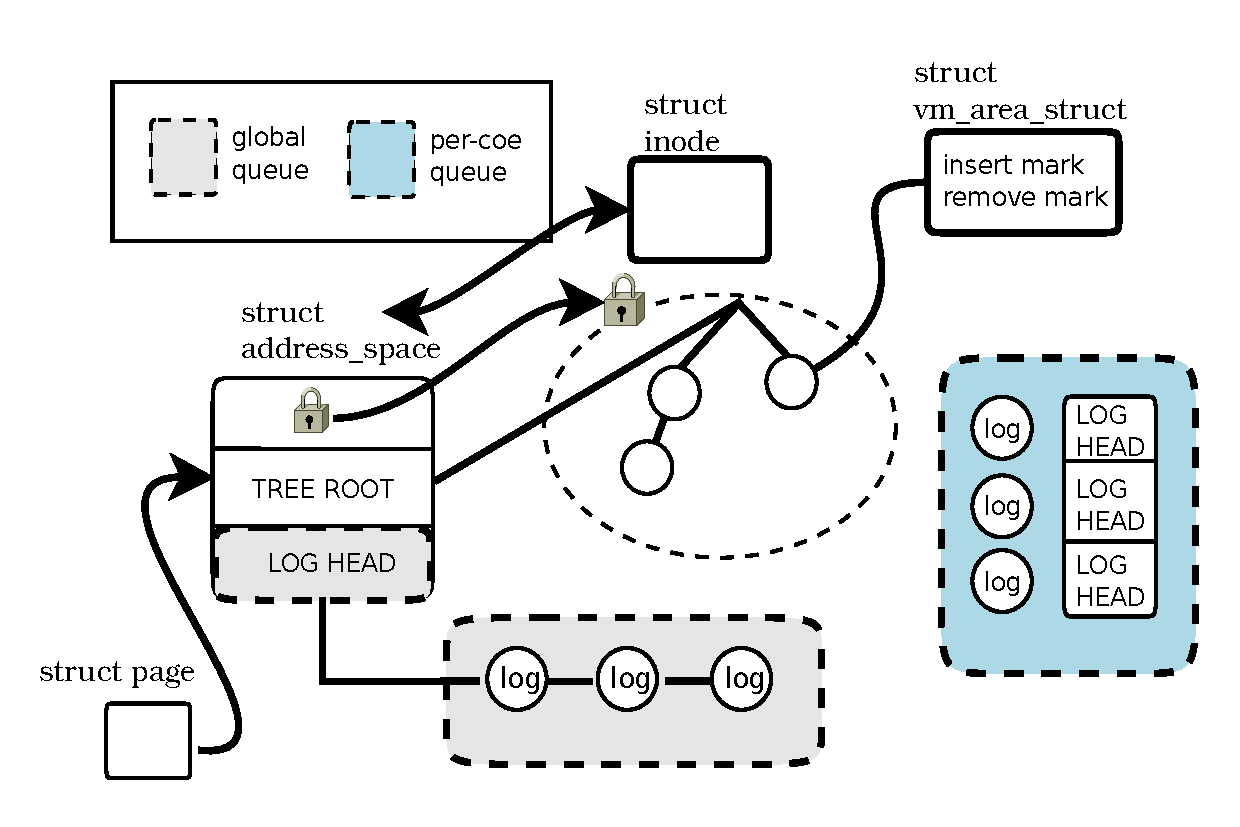
\includegraphics[width=0.5\textwidth]{fig/jaildocker}
  \end{center}
  \caption{The example showing seven update operations(insert C, insert D ,
  reader executes with lock.}
  \label{fig:basic}
\end{figure}


%$$$$$$$$$$$$$$$$$$$$$$$$$$$$$$$$$$$$$$$$$$$$$$$$$$$$$$$$$$$$$$$$$$$$$$$$$$$$$$$$
%$$$$$$$$$$$$$$$$$$$$$$$$$$$$$$$$$$$$$$$$$$$$$$$$$$$$$$$$$$$$$$$$$$$$$$$$$$$$$$$$
% 제안하는 구조 framework 설명
%$$$$$$$$$$$$$$$$$$$$$$$$$$$$$$$$$$$$$$$$$$$$$$$$$$$$$$$$$$$$$$$$$$$$$$$$$$$$$$$$
\ifkor
본 연구에서 제안하는 파티션닝 기반의 구조는 그림 <x>와 같다.
그림의 좌측은 우리가 제안하는 방법에 대한 프레임 워크를 보여주며, 오른쪽은 
파티션된 docker container들과 native로 동작하기 위한 구조를 보여주며, 마지막으로
소켓단위의 DRAM을 보여준다.
워크로드, 가용한 CPU 수 그리고 데이터 사이즈를 기반으로 파티션된 도커에서 수행할 지
아니면 native로 수행할 지 판단한다.
만약 사용 가능한 코어수가 작으면 SPARK는 적은 코어에서는 그림 <x-x>와 같이
Scalabe하므로 파티션된 도커 컨테이너에서 수행하지 않고, 그냥 Native로 수행한다.
그렇지 않다면, 데이터 사이즈가 설정된 heap 사이즈와 비교 후 Native로 실행 할 지
Docker에서 수행할지 판단한다.
만약 데이터 사이즈가 작은 경우는 native역시 scalable하므로 native 워커로 동작을 시킨다.
만약 데이터 사이즈가 큰 경우에는 파티션된 도커 워커에서 수행하는 것이 GC와 
NUMA의 영향과 operating system의 scalabilby 저해요소를 제거 할 수 있으므로 
파티션닝 기법으로 수행한다.
\else

\fi


%$$$$$$$$$$$$$$$$$$$$$$$$$$$$$$$$$$$$$$$$$$$$$$$$$$$$$$$$$$$$$$$$$$$$$$$$$$$$$$$$
%$$$$$$$$$$$$$$$$$$$$$$$$$$$$$$$$$$$$$$$$$$$$$$$$$$$$$$$$$$$$$$$$$$$$$$$$$$$$$$$$
% Docker를 이용하는 이유
%$$$$$$$$$$$$$$$$$$$$$$$$$$$$$$$$$$$$$$$$$$$$$$$$$$$$$$$$$$$$$$$$$$$$$$$$$$$$$$$$
\ifkor
우리는 Worker들의 파티션닝을 위해 Docker container를 사용하였다. 
그 이유는 virtual machine보다 훨씬 가벼운 구조로 되어 있으며, 
최근 docker기반으로 시스템을 관리하는 구조로 변경되고 있기 때문이다.
예를 들어 google kubernet을 사용할 경우, 워크마다 가장 최적의 파티션닝 값을 구한 후
그에 맞는 도커 컨테이너를 실행시키는 방법으로 구성하면 된다.
따라서 본 연구의 파티셔닝을 위한 방법으로 Docker container를 사용하였다.
\else

\fi


